\chapter{Hluboké Q-učení}

\section{Základní princip}
\subsection{Neuronová síť}

\subsection{Q-učení}
\subsection{Hluboké q-učení}

\section{Využití}
Kde se používá v praxi.


\section{Aplikace}
\subsection{Úvod}
Herní prostředí nám v každém kroku vrací i odměnu, kterou oba z hráčů za jejich akci obdrželi. Tuto informaci jsme v experimentech, provedených v rámci genetického programování, nevyužili, ale zde budou hrát velkou roli.

\subsection{Experiment 4: Soupeření s obranným agentem}
\begin{figure}[p]\centering
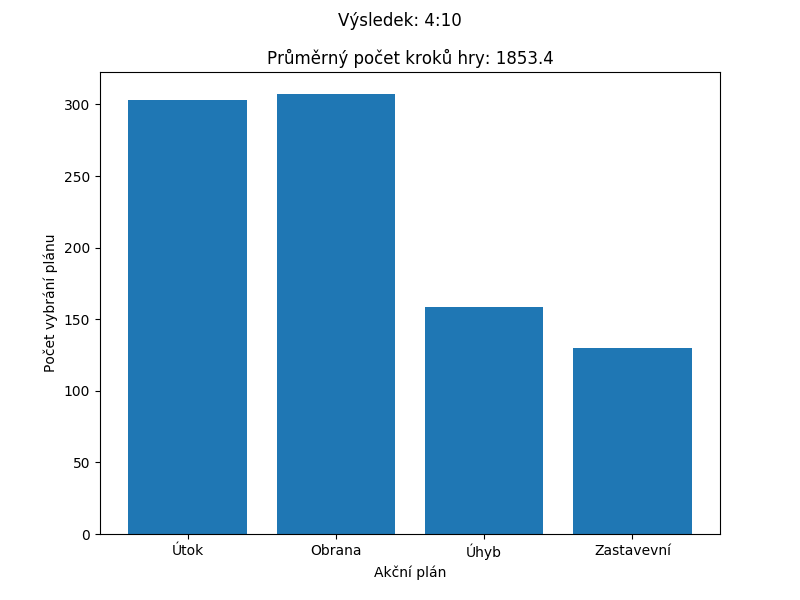
\includegraphics[width=145mm, height=110mm]{./Obrazky/Experiment04Results.png}
\caption{Výsledek experimentu 4}
\label{obr06:Výsledek experimentu 04}
\end{figure}

\subsection{Experiment 5: Elementární agent proti obrannému agentovi}
V tomto experimentu zkusíme sestoupit od abstrakcí v podobě akčních plánů k elementárním akcím a informacím o stavu.
I zde bude naším cílem trénování zadané neuronové sítě.
Tentokrát nebudeme neuronovou síť používat k volbě akčního plánu, ale přímo k volbě elementární akce.
Výsledný agent rozhodující se pomocí této neuronové sítě bude volit vždy jen jednu akci, proto nebudeme moci využít koncept přepočítávání akčních plánů a agent se bude rozhodovat v každém kroku.

\par
K pěti elementárním akcím přidáme navíc také možnost prázdné akce. Celkem tedy šest možností, proto naše neuronová síť bude mít právě šest výstupů.
Nebudeme volit akční plány, proto nemá ani dobrý smysl používat jejich délky jako vstupy, proto zde můžeme zvolit zcela jiný přístup.
Samotné simulace pro výpočet akčních plánů jsou výpočetně velmi náročné, tedy díky tomu, že zde zvolíme jednodušší přístup, tak budeme schopni, oproti předchozímu experimentu, zahrát v rámci trénování větší množství her.

\par
Vstupy neuronové sítě jsem si zvolil následující hodnoty:
\begin{itemize}
    \item Vektor pohybu vesmírné lodi
    \item Úhel natočení vesmírné lodi
    \item Počet uplynulých kroků od posledního výstřelu
    \item Relativní poloha nepřátelské lodi
    \item Relativní polohy tří nejbližších nebezpečných asteroidů
\end{itemize}

Jako nepřátelského agenta v tomto experimentu jsem zvolil agenta obranného.
Epsilon bylo nastaveno na 0.9985. Pro trénování bylo zahráno 10000 her.



% 10000_base_action_DQ_stable_deffensive_opponent_added_dense_layer_model_1
% 10000_base_action_DQ_stable_deffensive_opponent_added_dense_layer_1.txt

Výsledný agent proti obrannému agentovi nedopadl úspěšně. V souboji byl jednoznačně poražen se skóre 0:10.
V přehledu používaných akcí během souboje vidíme, že elementární agent používal v drtivé většině rotaci a střely.
To v praxi znamená, že se agent naučil točit dokola a kdykoliv může, tak vystřelit. Tato strategie skutečně přináší nějaké výsledky.
Agent tak rozstřeluje kolem letící asteroidy do všech různých směrů, avšak rozhoduje se pro toto chování bezmyšlenkovitě. Nemíří na žádné konkrétní asteroidy, ani na nepřátelskou loď.
Největší slabinou je, že agent se prakticky vůbec nenaučil bránit se. Zřejmě bylo v rámci trénování neuronové sítě nalezeno lokální optimum.

\begin{figure}[p]\centering
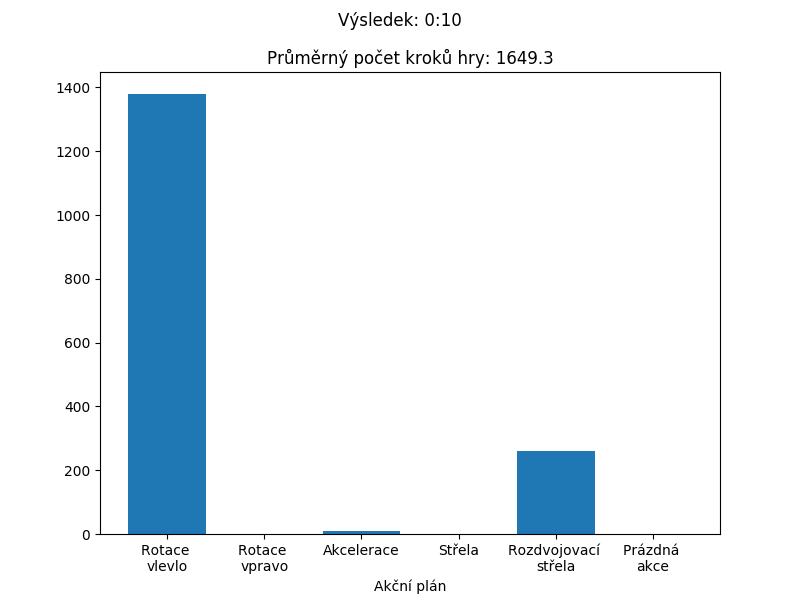
\includegraphics[width=145mm, height=110mm]{./Obrazky/Experiment05Results.png}
\caption{Výsledek experimentu 5}
\label{obr06:Výsledek experimentu 05}
\end{figure}
    



\subsection{Experiment 6: Dva elementární agenti}
Tento experiment rozšiřuje experiment předchozí. Budeme opět pracovat s elementárním agentem reprezentovaného neuronovou sítí stejného formátu jako v předhozím případě.
Tentokrát ale ale nebudeme v trénování hrát hry proti obrannému agentovi, nýbrž proti dalšímu elementárnímu agentovi, který bude také zároveň trénován.
Budeme tedy trénovat dvě neuronové sítě najednou. Teoreticky bychom měli dosáhnout vzájemného adaptivního učení, kde se každý z agentů snaží zlepšovat proti svému nepříteli a postupně se tak budou oba zlepšovat.
\par
Parametry trénování: ... 




,